\documentclass{article}
\usepackage[utf8]{inputenc}
\usepackage[T1]{fontenc}
\usepackage{lmodern}
\usepackage{geometry}
\geometry{margin=2cm}
\usepackage{graphicx}
\usepackage{hyperref}
\usepackage{listings}
\usepackage{xcolor}
\usepackage{float}
\usepackage{booktabs}
\usepackage{titling}
\usepackage{fancyhdr}
\usepackage{tcolorbox}
\usepackage{setspace}
\usepackage{titlesec}

% Enhanced typography
\onehalfspacing

% Define code listing style
\definecolor{codegreen}{rgb}{0,0.6,0}
\definecolor{codegray}{rgb}{0.5,0.5,0.5}
\definecolor{codepurple}{rgb}{0.58,0,0.82}
\definecolor{backcolour}{rgb}{0.95,0.95,0.95}

\lstdefinestyle{mystyle}{
    backgroundcolor=\color{backcolour},   
    commentstyle=\color{codegreen},
    keywordstyle=\color{blue},
    stringstyle=\color{codepurple},
    basicstyle=\ttfamily\small,
    breakatwhitespace=false,         
    breaklines=true,                 
    captionpos=b,                    
    keepspaces=true,                  
    showspaces=false,                
    showstringspaces=false,
    showtabs=false,                  
    tabsize=2,
    frame=single,
}

\lstset{style=mystyle}

% Hyperref setup
\hypersetup{
    colorlinks=true,
    linkcolor=blue,
    filecolor=magenta,
    urlcolor=blue,
    pdftitle={Court Kart: E-Commerce Database Implementation},
    pdfauthor={HADJ ARAB Adel},
    pdfsubject={E-Commerce Database},
    pdfkeywords={e-commerce, database, triggers, stored procedures, MySQL}
}

% Page style setup
\pagestyle{fancy}
\fancyhf{}
\fancyhead[R]{\thepage}
\fancyhead[L]{Court Kart E-Commerce}
\renewcommand{\headrulewidth}{0.4pt}

% Title formatting
\pretitle{\begin{center}\LARGE\bfseries}
\posttitle{\end{center}\vskip 0.5em}
\preauthor{\begin{center}\large}
\postauthor{\end{center}}
\predate{\begin{center}\large}
\postdate{\end{center}}

\renewcommand{\contentsname}{\centerline{TABLE OF CONTENTS}}

\begin{document}

% Custom title page
\begin{titlepage}
	\centering
	\vspace*{1cm}

	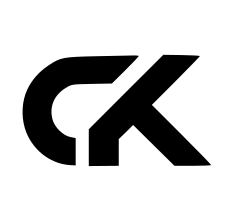
\includegraphics[width=0.4\textwidth]{../public/assets/images/court-kart-logo.png}\\[1.5cm]

	\textbf{\LARGE Court Kart: E-Commerce Platform}\\[0.5cm]
	\textbf{\Large PWEB and BDD Project}\\[2cm]

	\begin{minipage}{0.45\textwidth}
		\begin{flushleft}
			\large
			\textbf{Submitted by:}\\
			HADJ ARAB Adel\\
			Student ID: 222231482117\\
		\end{flushleft}
	\end{minipage}

	\vfill

	{\large \today}

\end{titlepage}

% Table of contents on separate page
\newpage
\tableofcontents
\newpage

\section{Introduction}

Court Kart is a specialized e-commerce platform designed for basketball enthusiasts, offering footwear, apparel, gear, and merchandise. The application follows the MVC (Model-View-Controller) architecture and implements features required for a complete online shopping experience. The platform provides a comprehensive solution for both customers and administrators, with features for inventory management, order processing, and user account management.

\section{Web Application Features}

\subsection{Main Shop Page Features}
The shop page implements all required features:
\begin{itemize}
	\item \textbf{Product display} with images, descriptions, and prices
	\item \textbf{Advanced search and filtering}:
	      \begin{itemize}
		      \item Text search (name, description)
		      \item Category filters
		      \item Price range filters
		      \item Sort options (price, popularity, newest)
	      \end{itemize}
	\item \textbf{Pagination} for browsing large product catalogs
	\item \textbf{Wishlist integration} for saving products
\end{itemize}

\begin{figure}[H]
	\centering
	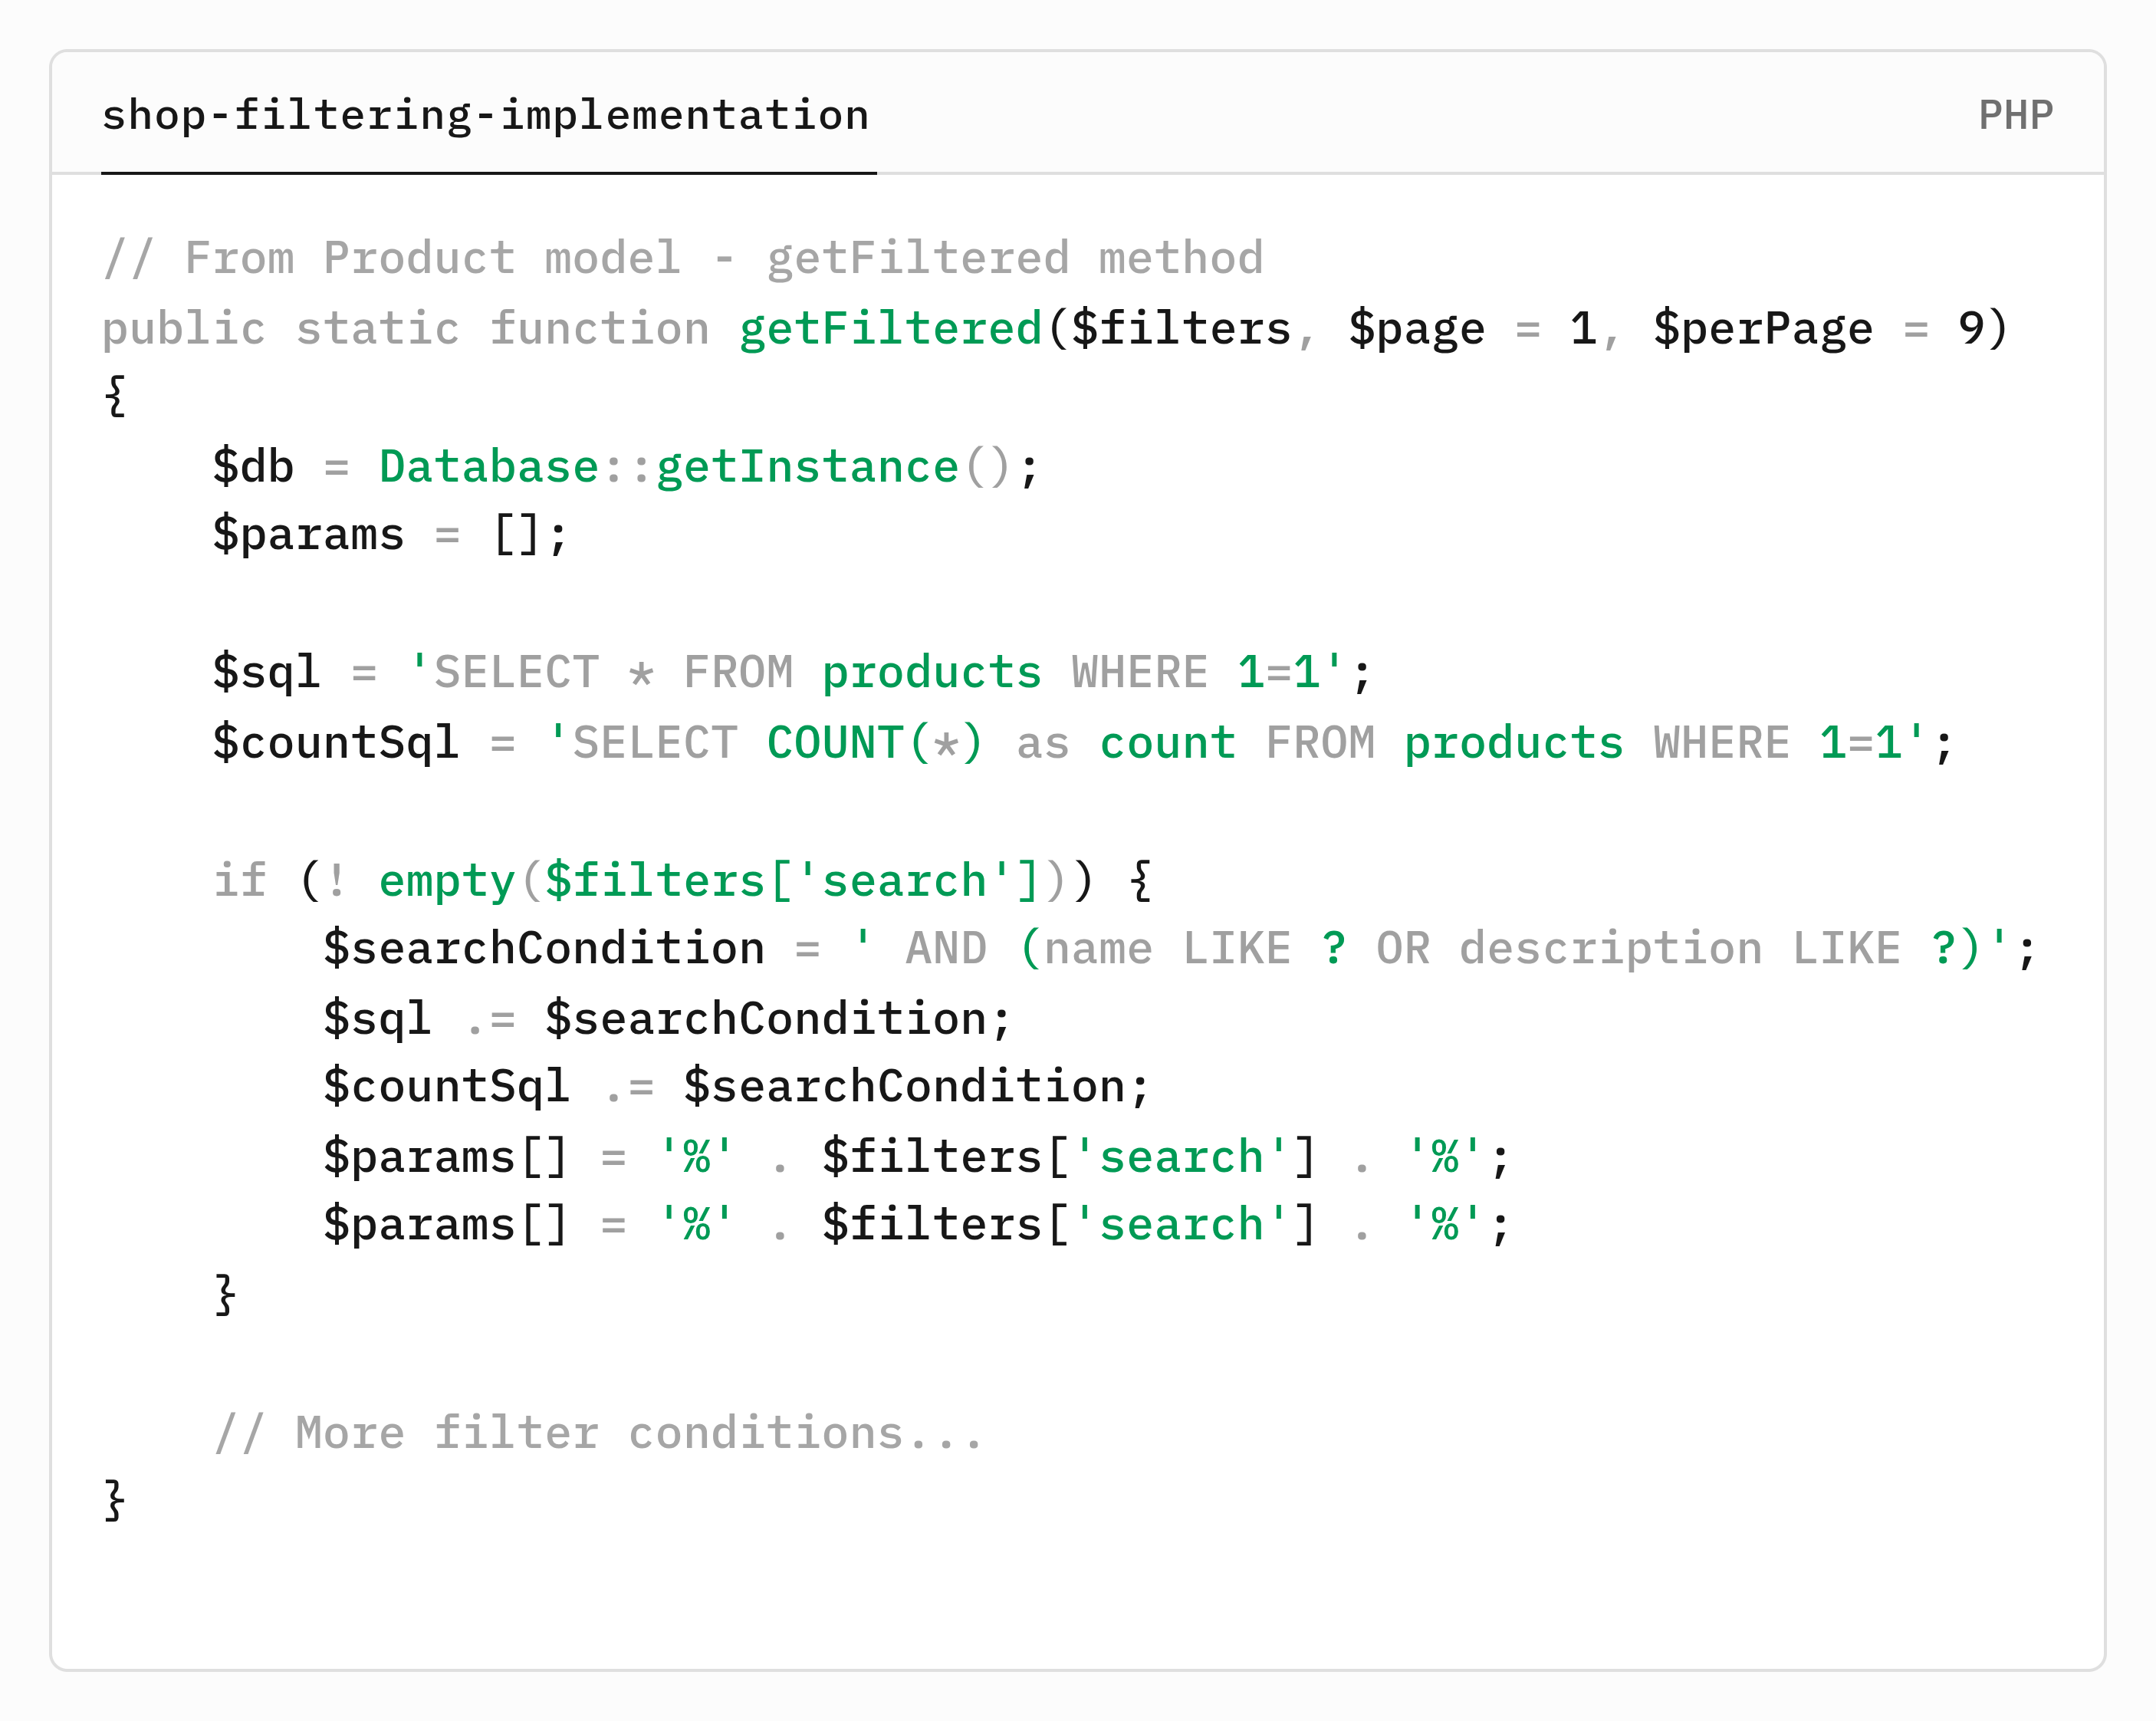
\includegraphics[width=0.7\textwidth]{images/shop-filtering-implementation.png}
	\caption{Shop Filtering Implementation}
\end{figure}


\subsection{User Features}
\begin{itemize}
	\item \textbf{User Authentication}: Secure login/logout with session management
	\item \textbf{Product Detail Views}: Complete product information, specifications, and reviews
	\item \textbf{Shopping Cart System}:
	      \begin{itemize}
		      \item Add/remove items
		      \item Update quantities
		      \item View cart state and totals
		      \item Session-based for guest users, database-synced for logged-in users
	      \end{itemize}
	\item \textbf{Order Tracking}: View status and history of placed orders
\end{itemize}

\begin{figure}[H]
	\centering
	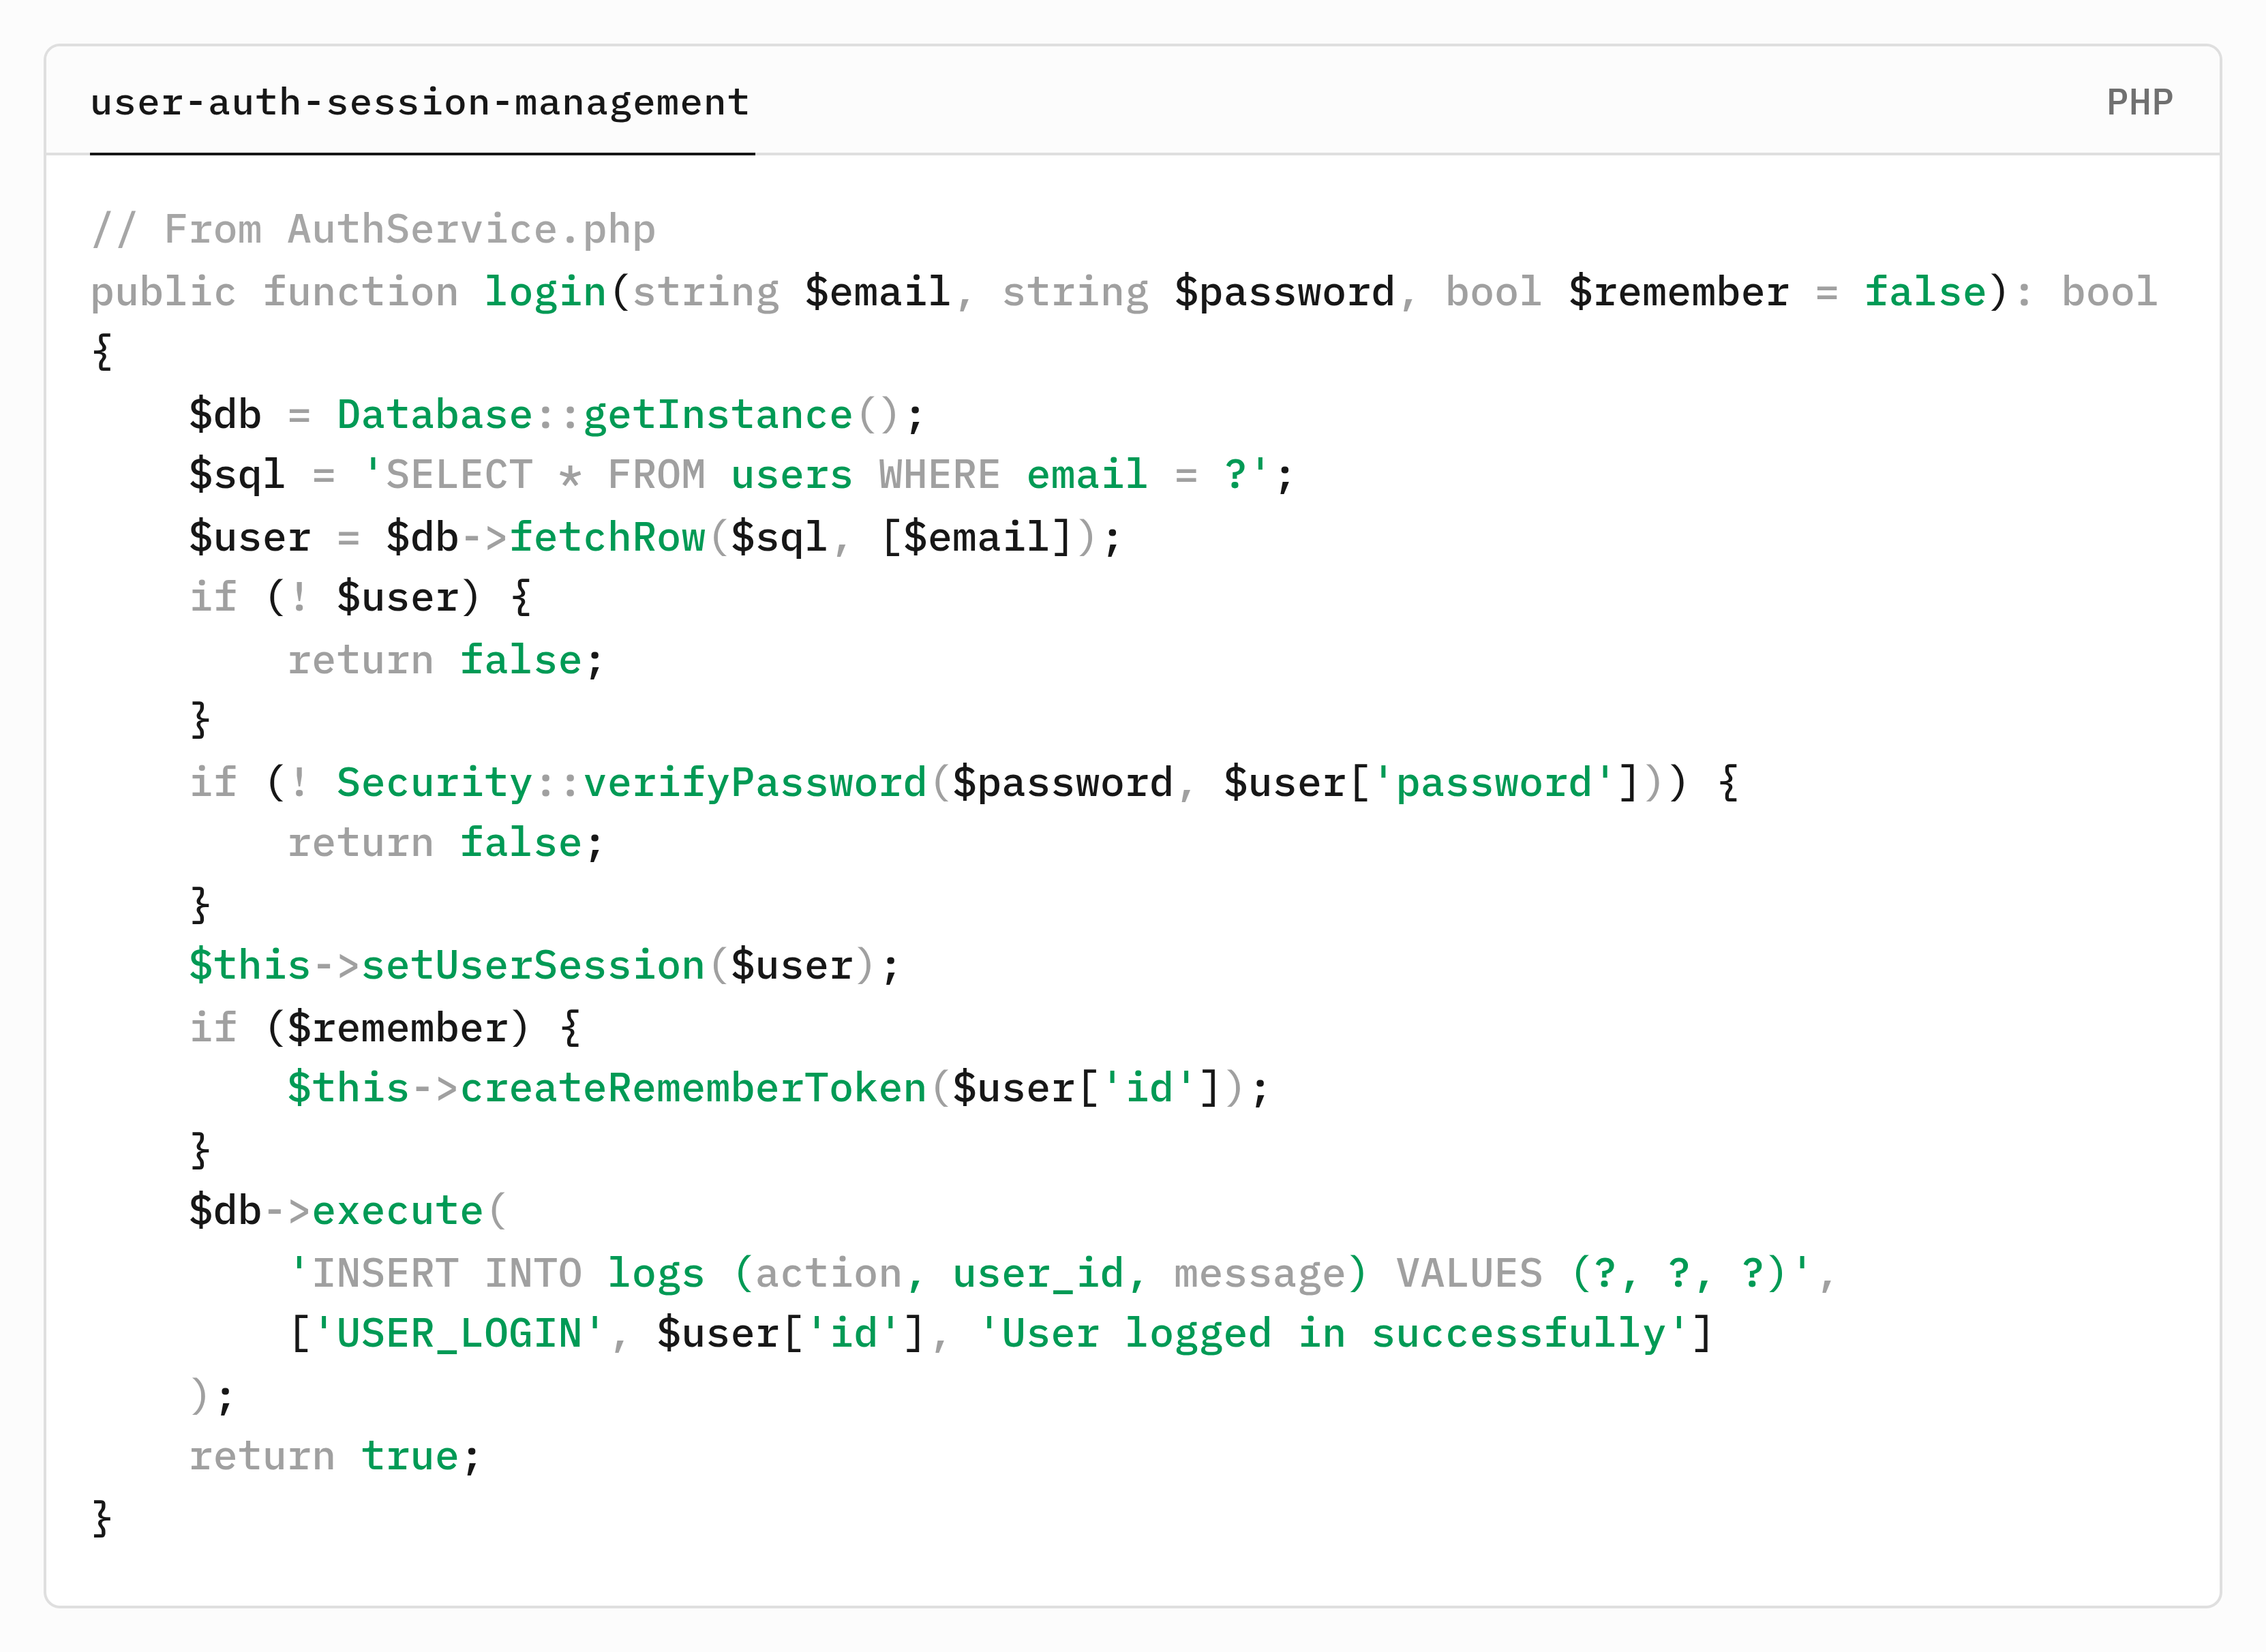
\includegraphics[width=0.8\textwidth]{images/user-auth-session-management.png}
	\caption{User Authentication with Session Management}
\end{figure}

\begin{lstlisting}[language=PHP, caption=Order tracking implementation]
// From OrderController.php
public function show($id)
{
    if (! Session::get('user_id')) {
        Session::flash('error', 'Please login to view your order');
        header('Location: /login');
        exit;
    }

    $userId = Session::get('user_id');
    $orderId = (int) $id;
    $orderDetails = Order::getOrderDetails($orderId);

    if (empty($orderDetails)) {
        Session::flash('error', 'Order not found');
        // Render error view...
        return;
    }

    if ($orderDetails[0]['user_id'] != $userId) {
        Session::flash('error', 'You do not have permission to view this order');
        // Render access denied view...
        return;
    }

    // Process order details and render view...
}
\end{lstlisting}

\subsection{Administrative Features}
An admin interface allows store management:
\begin{itemize}
	\item \textbf{Product Management}: Add, edit, delete products, update inventory
	\item \textbf{Order Processing}: View and update order status
	\item \textbf{Inventory Control}: Stock level monitoring with automatic alerts
\end{itemize}

\begin{lstlisting}[language=PHP, caption=Admin order status update]
// From AdminController.php
public function updateOrderStatus()
{
    if ($_SERVER['REQUEST_METHOD'] !== 'POST') {
        header('Location: /admin/orders');
        exit;
    }

    $orderId = $_POST['order_id'] ?? 0;
    $status = $_POST['status'] ?? '';

    if (! $orderId || ! $status) {
        Session::set('error', 'Invalid order ID or status');
        header('Location: /admin/orders');
        exit;
    }

    if (Order::updateStatus($orderId, $status)) {
        Session::set('success', 'Order status updated successfully');
    } else {
        Session::set('error', 'Failed to update order status');
    }

    header("Location: /admin/orders/{$orderId}");
    exit;
}
\end{lstlisting}

\begin{lstlisting}[language=PHP, caption=Admin middleware protection]
// From Middleware.php
public static function admin(): bool
{
    $authService = new AuthService;

    if (! $authService->isLoggedIn()) {
        Session::set('redirect_after_login', $_SERVER['REQUEST_URI']);
        header('Location: /login');
        exit;
    }

    if (! $authService->isAdmin()) {
        header('Location: /unauthorized');
        exit;
    }

    return true;
}
\end{lstlisting}

\section{Database Design}

\subsection{Relational Schema and Relationships}

Court Kart's database consists of the following key tables and relationships:

\begin{itemize}
	\item \textbf{users}: Stores authentication details and profile data
	      \begin{itemize}
		      \item One-to-many relationship with \texttt{orders} and \texttt{cart\_items}
	      \end{itemize}
	\item \textbf{products}: Contains product details including inventory levels and pricing
	      \begin{itemize}
		      \item Many-to-many with \texttt{orders} (via \texttt{order\_items})
		      \item Many-to-many with users' wishlists (via \texttt{wishlists})
	      \end{itemize}
	\item \textbf{cart\_items}: Links users to products in their cart
	      \begin{itemize}
		      \item Many-to-one relationship with \texttt{users} and \texttt{products}
	      \end{itemize}
	\item \textbf{orders}: Records transactions with status tracking
	      \begin{itemize}
		      \item Many-to-one relationship with \texttt{users}
		      \item One-to-many relationship with \texttt{order\_items}
		      \item One-to-one relationship with \texttt{canceled\_orders}
	      \end{itemize}
	\item \textbf{order\_items}: Contains line items within each order
	      \begin{itemize}
		      \item Many-to-one relationship with \texttt{orders} and \texttt{products}
	      \end{itemize}
	\item \textbf{canceled\_orders}: Records history and reasons for cancellations
	      \begin{itemize}
		      \item One-to-one relationship with \texttt{orders}
	      \end{itemize}
	\item \textbf{product\_reviews}: Stores customer ratings and reviews
	      \begin{itemize}
		      \item Many-to-one relationship with \texttt{products} and \texttt{users}
	      \end{itemize}
	\item \textbf{logs}: Maintains a comprehensive audit trail of operations
\end{itemize}

\begin{figure}[H]
	\centering
	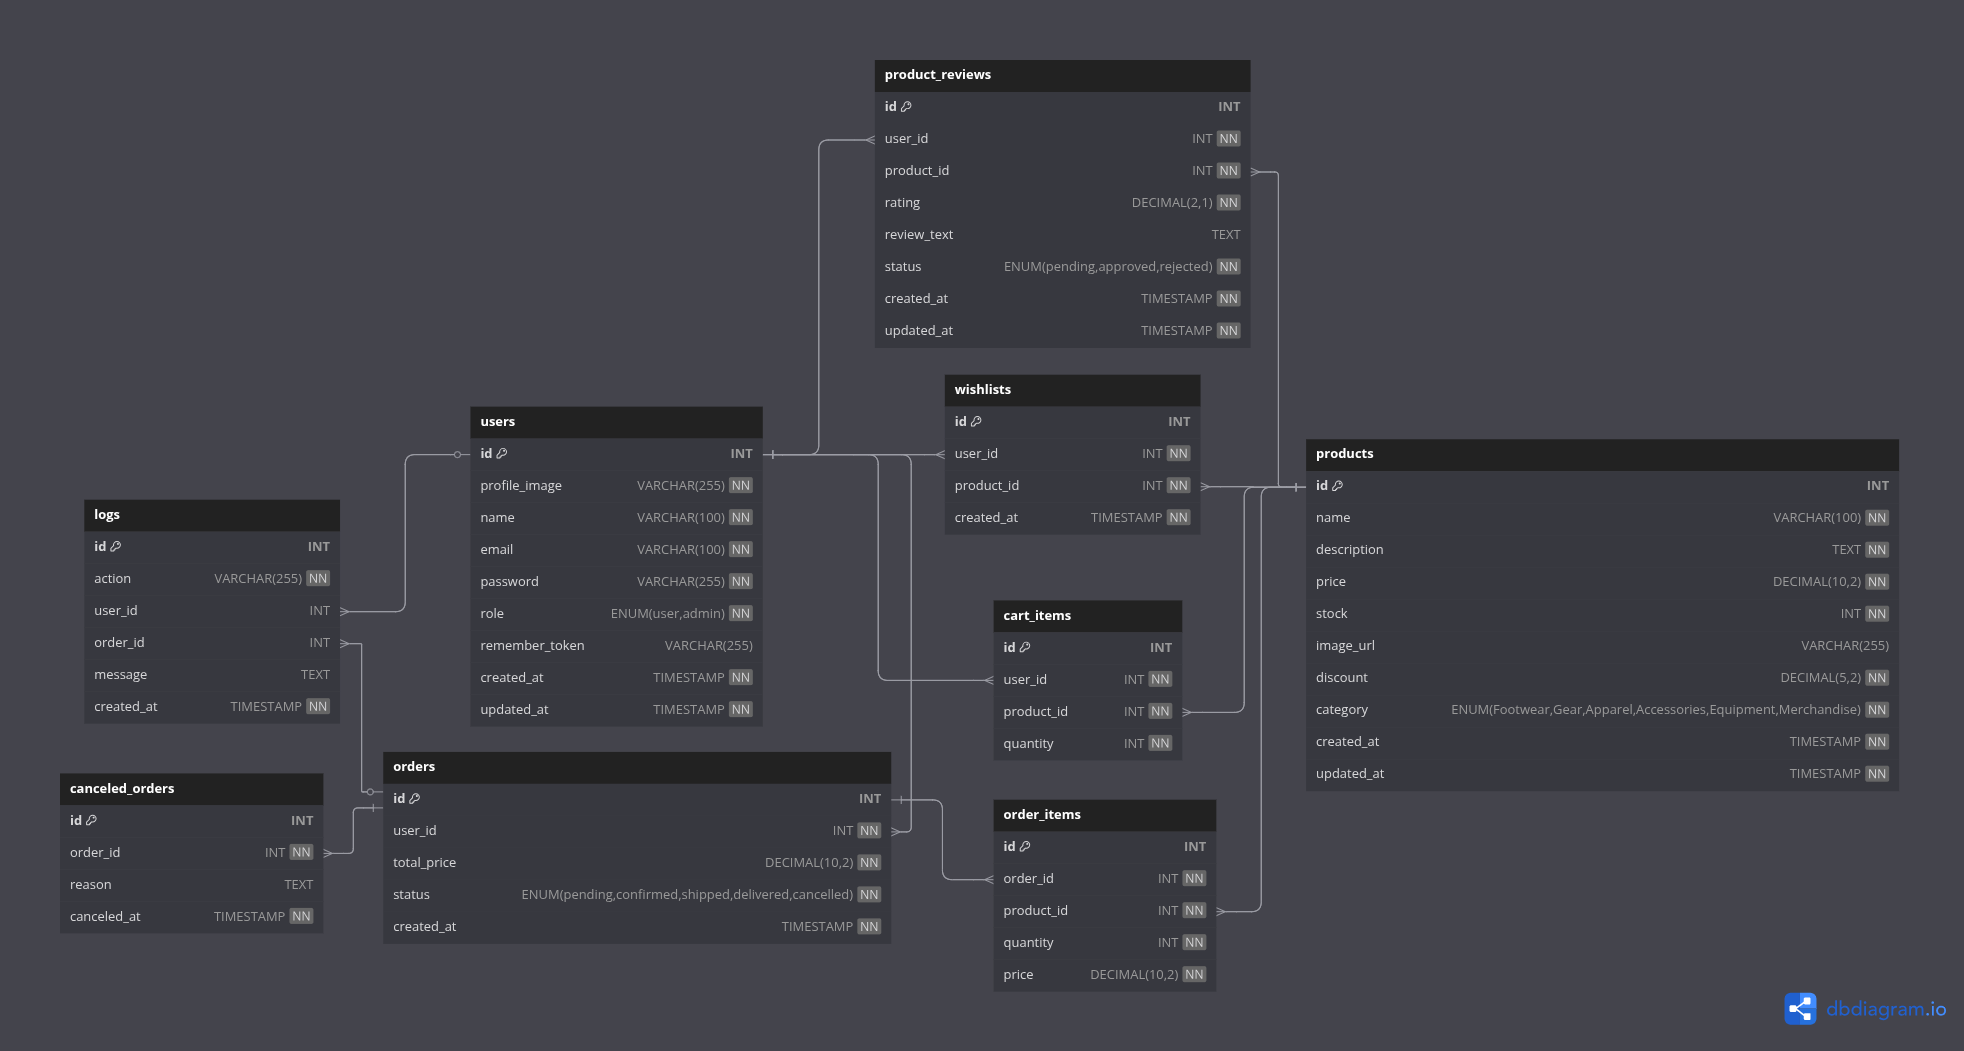
\includegraphics[width=0.9\textwidth]{../public/assets/images/db-schema.png}
	\caption{Court Kart Database Schema}
\end{figure}

\section{Stored Procedures Implementation}

\subsection{GetOrderDetails Procedure}
This procedure fulfills the requirement to display order details and total amount:

\begin{lstlisting}[language=SQL]
CREATE PROCEDURE GetOrderDetails (IN p_order_id INT)
BEGIN
    SELECT
        o.id AS order_id,
        o.created_at AS order_date,
        o.status,
        u.name AS customer_name,
        u.email AS customer_email,
        p.id AS product_id,
        p.name AS product_name,
        p.image_url,
        oi.quantity,
        oi.price AS unit_price,
        (oi.quantity * oi.price) AS subtotal,
        o.total_price AS total_amount
    FROM
        orders o
        JOIN users u ON o.user_id = u.id
        JOIN order_items oi ON o.id = oi.order_id
        JOIN products p ON oi.product_id = p.id
    WHERE
        o.id = p_order_id;
END
\end{lstlisting}

\subsection{FinalizeOrder Procedure}
This procedure finalizes an order and empties the cart once confirmed:

\begin{lstlisting}[language=SQL]
CREATE PROCEDURE FinalizeOrder (
    IN p_order_id INT,
    IN p_user_id INT
)
BEGIN
    DECLARE v_order_exists INT;

    START TRANSACTION;

    SELECT COUNT(*) INTO v_order_exists
    FROM orders
    WHERE id = p_order_id AND user_id = p_user_id AND status = 'pending';

    IF v_order_exists = 1 THEN
        UPDATE orders
        SET status = 'confirmed'
        WHERE id = p_order_id;

        DELETE FROM cart_items
        WHERE user_id = p_user_id;

        INSERT INTO logs (action, user_id, order_id, message)
        VALUES ('CHECKOUT', p_user_id, p_order_id, 'Order finalized and cart emptied');

        COMMIT;
    ELSE
        ROLLBACK;
        SIGNAL SQLSTATE '45000'
        SET MESSAGE_TEXT = 'Invalid or non-pending order for this user';
    END IF;
END
\end{lstlisting}

\subsection{GetCustomerOrderHistory Procedure}
This procedure displays a customer's order history:

\begin{lstlisting}[language=SQL]
CREATE PROCEDURE GetCustomerOrderHistory (
    IN p_user_id INT
)
BEGIN
    SELECT
        o.id AS order_id,
        o.created_at AS order_date,
        o.total_price,
        o.status,
        COUNT(oi.id) AS item_count,
        GROUP_CONCAT(p.name SEPARATOR ', ') AS products
    FROM
        orders o
        LEFT JOIN order_items oi ON o.id = oi.order_id
        LEFT JOIN products p ON oi.product_id = p.id
    WHERE
        o.user_id = p_user_id
    GROUP BY
        o.id, o.created_at, o.total_price, o.status
    ORDER BY
        o.created_at DESC;
END
\end{lstlisting}

\section{Triggers Implementation}

\subsection{AfterOrderConfirmed Trigger}
This trigger automatically updates product stock quantities when an order is confirmed:

\begin{lstlisting}[language=SQL]
CREATE TRIGGER AfterOrderConfirmed
AFTER UPDATE ON orders
FOR EACH ROW
BEGIN
    DECLARE v_done INT DEFAULT 0;
    DECLARE v_product_id INT;
    DECLARE v_quantity INT;
    DECLARE cur CURSOR FOR 
        SELECT product_id, quantity FROM order_items WHERE order_id = NEW.id;
    DECLARE CONTINUE HANDLER FOR NOT FOUND SET v_done = 1;

    IF OLD.status != 'confirmed' AND NEW.status = 'confirmed' THEN
        -- Log the order confirmation
        INSERT INTO logs (action, user_id, order_id, message)
        VALUES ('CHECKOUT', NEW.user_id, NEW.id, CONCAT('Order #', NEW.id, ' confirmed'));

        -- Update product stock using cursor
        OPEN cur;
        read_loop: LOOP
            FETCH cur INTO v_product_id, v_quantity;
            IF v_done THEN
                LEAVE read_loop;
            END IF;
            UPDATE products
            SET stock = stock - v_quantity
            WHERE id = v_product_id;
        END LOOP;
        CLOSE cur;
    END IF;
END
\end{lstlisting}

\subsection{BeforeOrderItemInsert Trigger}
This trigger prevents adding items to orders if the requested quantity exceeds available stock:

\begin{lstlisting}[language=SQL]
CREATE TRIGGER BeforeOrderItemInsert
BEFORE INSERT ON order_items
FOR EACH ROW
BEGIN
    DECLARE available_stock INT;
    DECLARE v_user_id INT;
    
    SELECT stock INTO available_stock
    FROM products
    WHERE id = NEW.product_id;
    
    SELECT user_id INTO v_user_id
    FROM orders
    WHERE id = NEW.order_id;

    IF NEW.quantity > available_stock THEN
        -- Log the stock limitation event
        INSERT INTO logs (action, user_id, order_id, message)
        VALUES ('PRODUCT_UPDATE', v_user_id, NEW.order_id, 
                CONCAT('Failed to add product #', NEW.product_id, 
                      ' to order #', NEW.order_id, 
                      ': Requested ', NEW.quantity, 
                      ', Available ', available_stock));
                
        SIGNAL SQLSTATE '45000'
        SET MESSAGE_TEXT = 'Cannot insert order item: requested quantity exceeds available stock';
    END IF;
END
\end{lstlisting}

\subsection{AfterOrderCancelled Trigger}
This trigger restores product stock when an order is canceled:

\begin{lstlisting}[language=SQL]
CREATE TRIGGER AfterOrderCancelled
AFTER UPDATE ON orders
FOR EACH ROW
BEGIN
    DECLARE v_done INT DEFAULT 0;
    DECLARE v_product_id INT;
    DECLARE v_quantity INT;
    DECLARE cur CURSOR FOR 
        SELECT product_id, quantity FROM order_items WHERE order_id = NEW.id;
    DECLARE CONTINUE HANDLER FOR NOT FOUND SET v_done = 1;

    IF OLD.status != 'cancelled' AND NEW.status = 'cancelled' THEN
        -- Log the order cancellation
        INSERT INTO logs (action, user_id, order_id, message)
        VALUES ('ORDER_CANCEL', NEW.user_id, NEW.id, 
                CONCAT('Order #', NEW.id, ' canceled'));
        
        -- Restore product stock using cursor
        OPEN cur;
        read_loop: LOOP
            FETCH cur INTO v_product_id, v_quantity;
            IF v_done THEN
                LEAVE read_loop;
            END IF;
            UPDATE products
            SET stock = stock + v_quantity
            WHERE id = v_product_id;
        END LOOP;
        CLOSE cur;
    END IF;
END
\end{lstlisting}

\subsection{LogCanceledOrder Trigger}
This trigger logs canceled orders into a history table:

\begin{lstlisting}[language=SQL]
CREATE TRIGGER LogCanceledOrder
AFTER UPDATE ON orders
FOR EACH ROW
BEGIN
    IF OLD.status != 'cancelled' AND NEW.status = 'cancelled' THEN
        -- Insert into cancellation history table
        INSERT INTO canceled_orders (order_id, reason, canceled_at)
        SELECT NEW.id, 'Order was canceled by user or admin', NOW()
        FROM dual
        WHERE NOT EXISTS (
            SELECT 1 FROM canceled_orders WHERE order_id = NEW.id
        );
        
        -- Log the cancellation record creation
        INSERT INTO logs (action, user_id, order_id, message)
        VALUES ('ORDER_CANCEL', NEW.user_id, NEW.id, 
                CONCAT('Order #', NEW.id, ' cancellation recorded'));
    END IF;
END
\end{lstlisting}

\section{Conclusion}
The Court Kart e-commerce platform successfully implements all required features specified in the project instructions:

\begin{itemize}
	\item A complete shop page with product listings and filters
	\item Detailed product views with descriptions and prices
	\item User authentication with session management
	\item Shopping cart functionality for adding/removing items
	\item Admin interface for managing products
	\item Database integration for all aspects of the application
	\item Stored procedures for order management and history
	\item Triggers for inventory control and order handling
\end{itemize}

The platform balances user experience with robust back-end functionality, creating a complete e-commerce solution for basketball enthusiasts while meeting all technical requirements.

\end{document}
